\documentclass[border=10pt]{standalone}

\usepackage{tikz}
\usepackage{tikzsymbols}
\usetikzlibrary{calc,patterns,shapes.geometric}

\def\centerarc[#1](#2)(#3:#4:#5){\draw[#1] ($(#2)+({#5*cos(#3)},{#5*sin(#3)})$) arc (#3:#4:#5);}

\begin{document}
	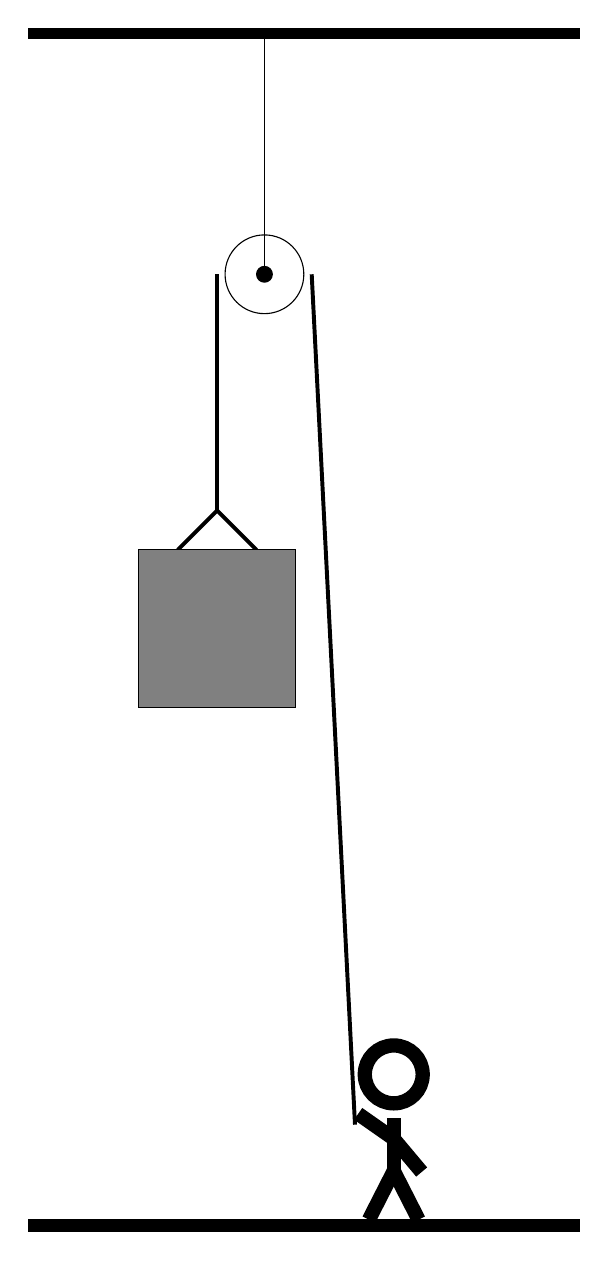
\begin{tikzpicture}
		%%%%% START %%%%%
		\draw[fill=black] (-2, 12) rectangle (5, 12.125);
		
		\draw (1, 9) circle (0.5);
		\draw[fill=black] (1, 9) circle (0.1);
		\draw (1, 12) -- (1, 9);
		
		\draw[line width=0.5mm] (-0.1, 5.5) -- (0.4, 6.0) -- (0.9, 5.5);
		\draw[fill=black!50] (-0.6, 5.5) rectangle (1.4, 3.5);
		
		\draw[line width=0.5mm] (0.4, 9) -- (0.4, 6.0);
		\centerarc[line width=0.5mm](1, 9)(0:180:0.6);
		\draw[line width=0.5mm](1.6, 9) -- (2.15, -1.8);
		
		\node at (2.6, -1.9) {\Strichmaxerl[10][-35][-50]};
		
		\draw[fill=black] (-2, -3) rectangle (5, -3.15);
		%%%%% END %%%%%
	\end{tikzpicture}
\end{document}